% Copyright 2019 by Till Tantau
%
% This file may be distributed and/or modified
%
% 1. under the LaTeX Project Public License and/or
% 2. under the GNU Free Documentation License.
%
% See the file doc/generic/pgf/licenses/LICENSE for more details.


\section{Transparency}
\label{section-tikz-transparency}

\subsection{Overview}

Normally, when you paint something using any of \tikzname's commands (this
includes stroking, filling, shading, patterns, and images), the newly painted
objects totally obscure whatever was painted earlier in the same area.

You can change this behavior by using something that can be thought of as
``(semi)transparent colors''. Such colors do not completely obscure the
background, rather they blend the background with the new color. At first
sight, using such semitransparent colors might seem quite straightforward, but
the math going on in the background is quite involved and the correct handling
of transparency fills some 64 pages in the PDF specification.

In the present section, we start with the different ways of specifying ``how
transparent'' newly drawn objects should be. The simplest way is to just
specify a percentage like ``60\% transparent''. A much more general way is to
use something that I call a \emph{fading}, also known as a soft mask or a mask.

At the end of the section we address the problem of creating so-called
\emph{transparency groups}. This problem arises when you paint over a position
several times with a semitransparent color. Sometimes you want the effect to
accumulate, sometimes you do not.

\emph{Note:} Transparency (or Opacity, as it may be called as well) is best
supported by the pdf\TeX\ driver. The \textsc{svg} driver also has some
support. The PostScript file format does not know about transparency. In
|dvips|-generated PostScript files, transparency of graphic objects is defined
through special commands that need further processing to become visible in the
\textsc{pdf} output. For this, a recent version of Ghostscript, preferably 9.52
or newer, is required and its command line utility |ps2pdf| must be called with
option |-dALLOWPSTRANSPARENCY|. Older versions may need option |-dNOSAFER|
instead, but some advanced features, such as \emph{transparency groups} and
\emph{fadings}, may not work at all. Printers and other programs will typically
ignore opacity settings in PostScript files.


\subsection{Specifying a Uniform Opacity}

Specifying a stroke and/or fill opacity is quite easy using the following
options.

\begin{key}{/tikz/draw opacity=\meta{value}}
    This option sets ``how transparent'' lines should be. A value of |1| means
    ``fully opaque'' or ``not transparent at all'', a value of |0| means
    ``fully transparent'' or ``invisible''. A value of |0.5| yields lines that
    are semitransparent.

    Note that when you use PostScript as your output format, this option works
    only with recent versions of Ghostscript.
    %
\begin{codeexample}[]
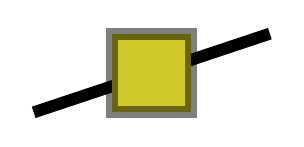
\begin{tikzpicture}[line width=1ex]
  \draw (0,0) -- (3,1);
  \filldraw [fill=yellow!80!black,draw opacity=0.5] (1,0) rectangle (2,1);
\end{tikzpicture}
\end{codeexample}
    %
\end{key}

Note that the |draw opacity| options only sets the opacity of drawn lines. The
opacity of fillings is set using the option |fill opacity| (documented in
Section~\ref{section-fill-opacity}. The option |opacity| sets both at the same
time.

\begin{key}{/tikz/opacity=\meta{value}}
    Sets both the drawing and filling opacity to \meta{value}.

    The following predefined styles make it easier to use this option:
    %
    \begin{stylekey}{/tikz/transparent}
        Makes everything totally transparent and, hence, invisible.
        %
\begin{codeexample}[]
\tikz{\fill[red]             (0,0)   rectangle (1,0.5);
      \fill[transparent,red] (0.5,0) rectangle (1.5,0.25); }
\end{codeexample}
    \end{stylekey}

    \begin{stylekey}{/tikz/ultra nearly transparent}
        Makes everything, well, ultra nearly transparent.
        %
\begin{codeexample}[]
\tikz{\fill[red]                      (0,0)   rectangle (1,0.5);
      \fill[ultra nearly transparent] (0.5,0) rectangle (1.5,0.25); }
\end{codeexample}
    \end{stylekey}

    \begin{stylekey}{/tikz/very nearly transparent}
\begin{codeexample}[]
\tikz{\fill[red]                     (0,0)   rectangle (1,0.5);
      \fill[very nearly transparent] (0.5,0) rectangle (1.5,0.25); }
\end{codeexample}
    \end{stylekey}

    \begin{stylekey}{/tikz/nearly transparent}
\begin{codeexample}[]
\tikz{\fill[red]                (0,0)   rectangle (1,0.5);
      \fill[nearly transparent] (0.5,0) rectangle (1.5,0.25); }
\end{codeexample}
    \end{stylekey}

    \begin{stylekey}{/tikz/semitransparent}
\begin{codeexample}[]
\tikz{\fill[red]             (0,0)   rectangle (1,0.5);
      \fill[semitransparent] (0.5,0) rectangle (1.5,0.25); }
\end{codeexample}
    \end{stylekey}

    \begin{stylekey}{/tikz/nearly opaque}
\begin{codeexample}[]
\tikz{\fill[red]           (0,0)   rectangle (1,0.5);
      \fill[nearly opaque] (0.5,0) rectangle (1.5,0.25); }
\end{codeexample}
    \end{stylekey}

    \begin{stylekey}{/tikz/very nearly opaque}
\begin{codeexample}[]
\tikz{\fill[red]                (0,0)   rectangle (1,0.5);
      \fill[very nearly opaque] (0.5,0) rectangle (1.5,0.25); }
\end{codeexample}
    \end{stylekey}

    \begin{stylekey}{/tikz/ultra nearly opaque}
\begin{codeexample}[]
\tikz{\fill[red]                 (0,0)   rectangle (1,0.5);
      \fill[ultra nearly opaque] (0.5,0) rectangle (1.5,0.25); }
\end{codeexample}
    \end{stylekey}

    \begin{stylekey}{/tikz/opaque}
        This yields completely opaque drawings, which is the default.
        %
\begin{codeexample}[]
\tikz{\fill[red]    (0,0)   rectangle (1,0.5);
      \fill[opaque] (0.5,0) rectangle (1.5,0.25); }
\end{codeexample}
    \end{stylekey}
\end{key}

\begin{key}{/tikz/fill opacity=\meta{value}}
    This option sets the opacity of fillings. In addition to filling
    operations, this opacity also applies to text and images.

    Note, again, that when you use PostScript as your output format, this
    option works only with recent versions of Ghostscript.
    %
\begin{codeexample}[]
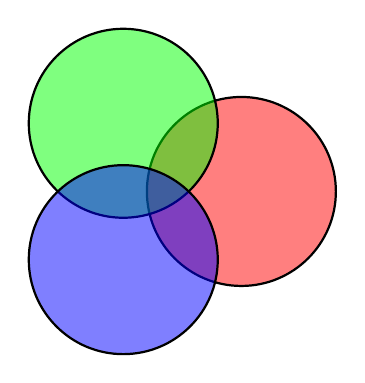
\begin{tikzpicture}[thick,fill opacity=0.5]
  \filldraw[fill=red]   (0:1cm)    circle (12mm);
  \filldraw[fill=green] (120:1cm)  circle (12mm);
  \filldraw[fill=blue]  (-120:1cm) circle (12mm);
\end{tikzpicture}
\end{codeexample}

\begin{codeexample}[]
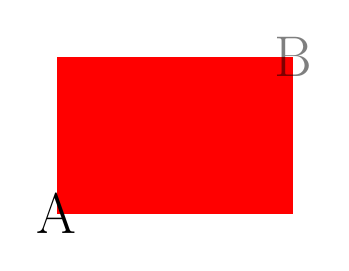
\begin{tikzpicture}
  \fill[red] (0,0) rectangle (3,2);

  \node                   at (0,0) {\huge A};
  \node[fill opacity=0.5] at (3,2) {\huge B};
\end{tikzpicture}
\end{codeexample}
    %
\end{key}

\begin{key}{/tikz/text opacity=\meta{value}}
    Sets the opacity of text labels, overriding the |fill opacity| setting.
    %
\begin{codeexample}[]
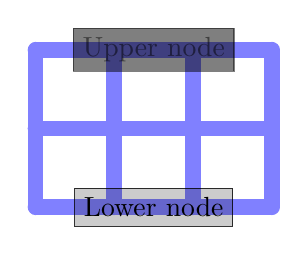
\begin{tikzpicture}[every node/.style={fill,draw}]
  \draw[line width=2mm,blue!50,line cap=round] (0,0) grid (3,2);

  \node[opacity=0.5] at (1.5,2) {Upper node};
  \node[draw opacity=0.8,fill opacity=0.2,text opacity=1]
    at (1.5,0) {Lower node};
\end{tikzpicture}
\end{codeexample}
    %
\end{key}

Note the following effect: If you set up a certain opacity for stroking or
filling and you stroke or fill the same area twice, the effect accumulates:
%
\begin{codeexample}[]
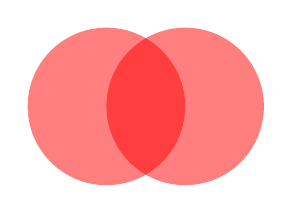
\begin{tikzpicture}[fill opacity=0.5]
  \fill[red] (0,0) circle (1);
  \fill[red] (1,0) circle (1);
\end{tikzpicture}
\end{codeexample}

Often, this is exactly what you intend, but not always. You can use
transparency groups, see the end of this section, to change this.


\subsection{Blend Modes}
\label{section-blend-modes}

A \emph{blend mode} specifies how colors mix when you paint on a canvas.
Normally, if you paint a red box on a green circle, the red color will
completely replace the green circle. However, in some situations you might also
wish the red color to somehow ``mix'' or ``blend'' with the green circle. We
already saw that, using transparency, we can draw something without completely
obscuring the background. \emph{Blending} is a similar operation, only here we
mix colors in more complicated ways.

\emph{Note:} Blending is a rather ``advanced'' feature of \textsc{pdf}. Most
renderers, let alone printers, will have trouble rendering blending correctly.

\begin{key}{/tikz/blend mode=\meta{mode}}
    Sets the current blend mode to \meta{mode}. Here \meta{mode} must be one of
    the modes listed below. More details on these modes can also be found in
    Section~7.2.4 of the \textsc{pdf} Specification, version~1.7.

    In the following example, the blend mode is only used and set inside a
    transparency group (see also Section~\ref{section-transparency-groups}).
    This is because most renderers (viewing programs) have trouble rendering
    blending correctly otherwise. For instance, at the time of writing, the
    versions of Adobe's Reader and Apple's Preview render the following drawing
    very differently, if the transparency group is not used in the following
    example.
    %
\begin{codeexample}[]
\tikz {
  \begin{scope}[transparency group]
    \begin{scope}[blend mode=screen]
      \fill[red!90!black]   ( 90:.6) circle (1);
      \fill[green!80!black] (210:.6) circle (1);
      \fill[blue!90!black]  (330:.6) circle (1);
    \end{scope}
  \end{scope}
}
\end{codeexample}

    Because of the trouble with rendering blending correctly outside
    transparency groups, there is a special key that establishes a transparency
    group and sets a blend mode simultaneously:

    \begin{key}{/tikz/blend group=\meta{mode}}
        This key can only be used with a scope (like |transparency group|). It
        will cause the current scope to become a transparency group and, inside
        this group, the blend mode will be set to \meta{mode}.
        %
\begin{codeexample}[]
\tikz [blend group=screen] {
  \fill[red!90!black]   ( 90:.6) circle (1);
  \fill[green!80!black] (210:.6) circle (1);
  \fill[blue!90!black]  (330:.6) circle (1);
}
\end{codeexample}
    \end{key}

    Here is an overview of the effects of the different available blend modes.
    In the examples, we always have three circles drawn on top of each other
    (as in the example code earlier): We start with a triple of pure red,
    green, and blue. Below it, we have a triple of light versions of these
    three colors (|red!50|, |green!50|, and |blue!50|). Next comes the triple
    yellow, cyan, and magenta; again with a triple of light versions below it.
    The large example consists of three balls (produced using |ball color|)
    having the colors red, green, and blue, are drawn on top of each other just
    like the circles.

    \definecolor{rg}{rgb}{1,1,0}
    \definecolor{gb}{rgb}{0,1,1}
    \definecolor{br}{rgb}{1,0,1}

    \def\makeline#1#2#3{\leavevmode
        \hbox to 40mm{#1\hss}\ \hbox to
        20.5mm{#2\hss}\ \begin{minipage}[t]{88.5mm}\raggedright#3\end{minipage}\par
        \textcolor{black!25}{\hrule height1pt}
    }

    \def\showmode#1#2{
        \makeline{
            \tikz [blend mode=#1,baseline=-.5ex] {
              \fill[red]      ( 90:.5em) circle (.75em);
              \fill[green]    (210:.5em) circle (.75em);
              \fill[blue]     (330:.5em) circle (.75em);
              \scoped[yshift=-2.5em]{
                \fill[red!50]   ( 90:.5em) circle (.75em);
                \fill[green!50] (210:.5em) circle (.75em);
                \fill[blue!50]  (330:.5em) circle (.75em);
              }
            }
            \tikz [blend mode=#1,baseline=-.5ex] {
              \fill[rg]       ( 90:.5em) circle (.75em);
              \fill[gb]       (210:.5em) circle (.75em);
              \fill[br]       (330:.5em) circle (.75em);
              \scoped[yshift=-2.5em]{
                \fill[rg!50]  ( 90:.5em) circle (.75em);
                \fill[gb!50]  (210:.5em) circle (.75em);
                \fill[br!50]  (330:.5em) circle (.75em);
              }
            }
            \tikz [blend mode=#1,baseline=-.5ex+1.25em] {
              \shade[ball color=red]   ( 90:1em) circle (1.5em);
              \shade[ball color=green] (210:1em) circle (1.5em);
              \shade[ball color=blue]  (330:1em) circle (1.5em);
            }}{\verb|#1|}{#2}%
               % this argument was changed from {|#1|}
               % --> see <https://sourceforge.net/p/pgf/bugs/486/>
    }

    \medskip
    \makeline{\emph{Example}}{\emph{Mode}}{\emph{Explanations quoted from
        Table~7.2 of the \textsc{pdf} Specification, Version~1.7}}
    \showmode{normal}{When painting a pixel with a some color (called the
        ``source color''), the background color (called the ``backdrop'') is
        completely ignored.}
    \showmode{multiply}{Multiplies the backdrop and source color values. The
        result color is always at least as dark as either of the two
        constituent colors. Multiplying any color with black produces black;
        multiplying with white leaves the original color unchanged. Painting
        successive overlapping objects with a color other than black or white
        produces progressively darker colors.}
    \showmode{screen}{Multiplies the complements of the backdrop and source
        color values, then complements the result. The result color is always
        at least as light as either of the two constituent colors. Screening
        any color with white produces white; screening with black leaves the
        original color unchanged. The effect is similar to projecting multiple
        photographic slides simultaneously onto a single screen.}
    \showmode{overlay}{Multiplies or screens the colors, depending on the
        backdrop color value. Source colors overlay the backdrop while
        preserving its highlights and shadows. The backdrop color is not
        replaced but is mixed with the source color to reflect the lightness or
        darkness of the backdrop.}
    \showmode{darken}{Selects the darker of the backdrop and source colors. The
        backdrop is replaced with the source where the source is darker;
        otherwise, it is left unchanged.}
    \showmode{lighten}{Selects the lighter of the backdrop and source colors.
        The backdrop is replaced with the source where the source is lighter;
        otherwise, it is left unchanged.}
    \showmode{color dodge}{Brightens the backdrop color to reflect the source
        color. Painting with black produces no changes.}
    \showmode{color burn}{Darkens the backdrop color to reflect the source
        color. Painting with white produces no change.}
    \showmode{hard light}{Multiplies or screens the colors, depending on the
        source color value. The effect is similar to shining a harsh spotlight
        on the backdrop.}
    \showmode{soft light}{Darkens or lightens the colors, depending on the
        source color value. The effect is similar to shining a diffused
        spotlight on the backdrop.}
    \showmode{difference}{Subtracts the darker of the two constituent colors
        from the lighter color. Painting with white inverts the backdrop color;
        painting with black produces no change.}
    \showmode{exclusion}{Produces an effect similar to that of the Difference
        mode but lower in contrast. Painting with white inverts the backdrop
        color; painting with black produces no change.}
    \showmode{hue}{Creates a color with the hue of the source color and the
        saturation and luminosity of the backdrop color.}
    \showmode{saturation}{Creates a color with the saturation of the source
        color and the hue and luminosity of the backdrop color. Painting with
        this mode in an area of the backdrop that is a pure gray (no
        saturation) produces no change.}
    \showmode{color}{Creates a color with the hue and saturation of the source
        color and the luminosity of the backdrop color. This preserves the gray
        levels of the backdrop and is useful for coloring monochrome images or
        tinting color images.}
    \showmode{luminosity}{Creates a color with the luminosity of the source
        color and the hue and saturation of the backdrop color. This produces
        an inverse effect to that of the Color mode.}
\end{key}


\subsection{Fadings}

For complicated graphics, uniform transparency settings are not always
sufficient. Suppose, for instance, that while you paint a picture, you want the
transparency to vary smoothly from completely opaque to completely transparent.
This is a ``shading-like'' transparency. For such a form of transparency I will
use the term \emph{fading} (as a noun). They are also known as \emph{soft
masks}, \emph{opacity masks}, \emph{masks}, or \emph{soft clips}.


\subsubsection{Creating Fadings}

How do we specify a fading? This is a bit of an art since the underlying
mechanism is quite powerful, but a bit difficult to use.

Let us start with a bit of terminology. A \emph{fading} specifies for each
point of an area the transparency of that point. This transparency can by any
number between 0 and 1. A \emph{fading picture} is a normal graphic that, in a
way to be described in a moment, determines the transparency of points inside
the fading. Each fading has an underlying fading picture.

The fading picture is a normal graphic drawn using any of the normal graphic
drawing commands. A fading and its fading picture are related as follows: Given
any point of the fading, the transparency of this point is determined by the
luminosity of the fading picture at the same position. The luminosity of a
point determines ``how bright'' the point is. The brighter the point in the
fading picture, the more opaque is the point in the fading. In particular, a
white point of the fading picture is completely opaque in the fading and a
black point of the fading picture is completely transparent in the fading. (The
background of the fading picture is always transparent in the fading as if the
background were black.)

It is rather counter-intuitive that a \emph{white} pixel of the fading picture
will be \emph{opaque} in the fading and a \emph{black} pixel will be
\emph{transparent}. For this reason, \tikzname\ defines a color called
|transparent| that is the same as |black|. The nice thing about this definition
is that the color |transparent!|\meta{percentage} in the fading picture yields
a pixel that is \meta{percentage} percent transparent in the fading.

Turning a fading picture into a normal picture is achieved using the following
commands, which are \emph{only defined in the library}, namely the library
|fadings|. So, to use them, you have to say |\usetikzlibrary{fadings}| first.

\begin{environment}{{tikzfadingfrompicture}\oarg{options}}
    This command works like a |{tikzpicture}|, only the picture is not shown,
    but instead a fading is defined based on this picture. To set the name of
    the picture, use the |name| option (which is normally used to set the name
    of a node).
    %
    \begin{key}{/tikz/name=\marg{name}}
        Use this option with the |{tikzfadingfrompicture}| environment to set
        the name of the fading. You \emph{must} provide this option.
    \end{key}

    The following shading is 2cm by 2cm and gets more and more transparent from
    left to right, but is 50\% transparent for a large circle in the middle.
    %
{\ifpgfmanualexternalize\tikzexternaldisable\fi
\begin{codeexample}[preamble={\usetikzlibrary{fadings,patterns}}]
\begin{tikzfadingfrompicture}[name=fade right with circle]
  \shade[left color=transparent!0,
         right color=transparent!100] (0,0) rectangle (2,2);
  \fill[transparent!50] (1,1) circle (0.7);
\end{tikzfadingfrompicture}

% Now we use the fading in another picture:
\begin{tikzpicture}
  % Background
  \fill [black!20] (-1.2,-1.2) rectangle (1.2,1.2);
  \pattern [pattern=checkerboard,pattern color=black!30]
                   (-1.2,-1.2) rectangle (1.2,1.2);

  \fill [path fading=fade right with circle,red] (-1,-1) rectangle (1,1);
\end{tikzpicture}
\end{codeexample}
    %
    In the next example we create a fading picture that contains some text.
    When the fading is used, we only see the shading ``through it''.
    %
\begin{codeexample}[preamble={\usetikzlibrary{fadings,patterns}}]
\begin{tikzfadingfrompicture}[name=tikz]
  \node [text=transparent!20]
  {\fontencoding{T1}\fontfamily{ptm}\fontsize{45}{45}\bfseries\selectfont
    Ti\emph{k}Z};
\end{tikzfadingfrompicture}

% Now we use the fading in another picture:
\begin{tikzpicture}
  \fill [black!20] (-2,-1) rectangle (2,1);
  \pattern [pattern=checkerboard,pattern color=black!30]
                   (-2,-1) rectangle (2,1);

  \shade[path fading=tikz,fit fading=false,
         left color=blue,right color=black]
    (-2,-1) rectangle (2,1);
\end{tikzpicture}
\end{codeexample}
}%

    The same effect can also be achieved using knockout groups, see
    Section~\ref{section-transparency-groups}.
\end{environment}

\begin{plainenvironment}{{tikzfadingfrompicture}\oarg{options}}
    The plain\TeX\ version of the environment.
\end{plainenvironment}

\begin{contextenvironment}{{tikzfadingfrompicture}\oarg{options}}
    The Con\TeX t version of the environment.
\end{contextenvironment}

\begin{command}{\tikzfading\oarg{options}}
    This command is used to define a fading similarly to the way a shading is
    defined. In the \meta{options} you should
    %
    \begin{enumerate}
        \item use the |name=|\meta{name} option to set a name for the fading,
        \item use the |shading| option to set the name of the shading that you
            wish to use,
        \item extra options for setting the colors of the shading (typically
            you will set them to the color |transparent!|\meta{percentage}).
    \end{enumerate}
    %
    Then, a new fading named \meta{name} will be created based on the shading.
    %
\begin{codeexample}[preamble={\usetikzlibrary{fadings,patterns}}]
\tikzfading[name=fade right,
            left color=transparent!0,
            right color=transparent!100]

% Now we use the fading in another picture:
\begin{tikzpicture}
  % Background
  \fill [black!20] (-1.2,-1.2) rectangle (1.2,1.2);
  \path [pattern=checkerboard,pattern color=black!30]
                   (-1.2,-1.2) rectangle (1.2,1.2);

  \fill [red,path fading=fade right] (-1,-1) rectangle (1,1);
\end{tikzpicture}
\end{codeexample}

\begin{codeexample}[preamble={\usetikzlibrary{fadings,patterns}}]
\tikzfading[name=fade out,
            inner color=transparent!0,
            outer color=transparent!100]

% Now we use the fading in another picture:
\begin{tikzpicture}
  % Background
  \fill [black!20] (-1.2,-1.2) rectangle (1.2,1.2);
  \path [pattern=checkerboard,pattern color=black!30]
                   (-1.2,-1.2) rectangle (1.2,1.2);

  \fill [blue,path fading=fade out] (-1,-1) rectangle (1,1);
\end{tikzpicture}
\end{codeexample}
    %
\end{command}


\subsubsection{Fading a Path}

A fading specifies for each pixel of a certain area how transparent this pixel
will be. The following options are used to install such a fading for the
current scope or path.

\pgfdeclarefading{fade down}{%
  \tikzset{top color=pgftransparent!0,bottom color=pgftransparent!100}
  \pgfuseshading{axis}
}
\pgfdeclarefading{fade inside}{%
  \tikzset{inner color=pgftransparent!90,outer color=pgftransparent!30}
  \pgfuseshading{radial}
}

\begin{key}{/tikz/path fading=\meta{name} (default \normalfont scope's setting)}
    This option tells \tikzname\ that the current path should be faded with the
    fading \meta{name}. If no \meta{name} is given, the \meta{name} set for the
    whole scope is used. Similarly to options like |draw| or |fill|, this
    option is reset for each path, so you have to add it to each path that
    should be faded. You can also specify |none| as \meta{name}, in which case
    fading for the path will be switched off in case it has been switched on by
    previous options or styles.
    %
\begin{codeexample}[preamble={\usetikzlibrary{fadings,patterns}}]
\begin{tikzpicture}[path fading=south]
  % Checker board
  \fill [black!20] (0,0) rectangle (4,3);
  \pattern [pattern=checkerboard,pattern color=black!30]
                   (0,0) rectangle (4,3);

  \fill [color=blue]                   (0.5,1.5) rectangle +(1,1);
  \fill [color=blue,path fading=north] (2.5,1.5) rectangle +(1,1);

  \fill [color=red,path fading]        (1,0.75) ellipse (.75 and .5);
  \fill [color=red]                    (3,0.75) ellipse (.75 and .5);
\end{tikzpicture}
\end{codeexample}

    \begin{key}{/tikz/fit fading=\meta{boolean} (default true, initially true)}
        When set to |true|, the fading is shifted and resized (in exactly the
        same way as a shading) so that it covers the current path. When set to
        |false|, the fading is only shifted so that it is centered on the
        path's center, but it is not resized. This can be useful for
        special-purpose fadings, for instance when you use a fading to ``punch
        out'' something.
    \end{key}

    \begin{key}{/tikz/fading transform=\meta{transformation options}}
        The \meta{transformation options} are applied to the fading before it
        is used. For instance, if \meta{transformation options} is set to
        |rotate=90|, the fading is rotated by 90 degrees.
        %
\begin{codeexample}[
    preamble={\usetikzlibrary{fadings,patterns}},
    pre={\pgfdeclarefading{fade down}{%
  \tikzset{top color=pgftransparent!0,bottom color=pgftransparent!100}
  \pgfuseshading{axis}
}}]
\begin{tikzpicture}[path fading=fade down]
  % Checker board
  \fill [black!20] (0,0) rectangle (4,1.5);
  \path [pattern=checkerboard,pattern color=black!30] (0,0) rectangle (4,1.5);

  \fill [red,path fading,fading transform={rotate=90}]
    (1,0.75) ellipse (.75 and .5);
  \fill [red,path fading,fading transform={rotate=30}]
    (3,0.75) ellipse (.75 and .5);
\end{tikzpicture}
\end{codeexample}
    \end{key}

    \begin{key}{/tikz/fading angle=\meta{degree}}
        A shortcut for |fading transform={rotate=|\meta{degree}|}|.
    \end{key}

    Note that you can ``fade just about anything''. In particular, you can fade
    a shading.
    %
\begin{codeexample}[preamble={\usetikzlibrary{fadings,patterns}}]
\begin{tikzpicture}
  % Checker board
  \fill [black!20] (0,0) rectangle (4,4);
  \path [pattern=checkerboard,pattern color=black!30] (0,0) rectangle (4,4);

  \shade [ball color=blue,path fading=south] (2,2) circle (1.8);
\end{tikzpicture}
\end{codeexample}

    The |fade inside| of the following example is more transparent in the
    middle than on the outside.
    %
\begin{codeexample}[preamble={\usetikzlibrary{fadings,patterns}}]
\tikzfading[name=fade inside,
            inner color=transparent!80,
            outer color=transparent!30]
\begin{tikzpicture}
  % Checker board
  \fill [black!20] (0,0) rectangle (4,4);
  \path [pattern=checkerboard,pattern color=black!30] (0,0) rectangle (4,4);

  \shade [ball color=red] (3,3) circle (0.8);
  \shade [ball color=white,path fading=fade inside] (2,2) circle (1.8);
\end{tikzpicture}
\end{codeexample}

    Note that adding the |path fading| option to a node fades the (background)
    path, not the text itself. To fade the text, you need to use a scope fading
    (see below).
\end{key}

Note that using fadings in conjunction with patterns can create visually rather
pleasing effects:
%
\begin{codeexample}[preamble={\usetikzlibrary{fadings,patterns,shadows}}]
\tikzfading[name=middle,
            top color=transparent!50,
            bottom color=transparent!50,
            middle color=transparent!20]
\begin{tikzpicture}
  \node      [circle,circular drop shadow,
              pattern=horizontal lines dark blue,
              path fading=south,
              minimum size=3.6cm] {};
  \pattern   [path fading=north,
              pattern=horizontal lines dark gray]
    (0,0) circle (1.8cm);
  \pattern   [path fading=middle,
              pattern=crosshatch dots light steel blue]
    (0,0) circle (1.8cm);
\end{tikzpicture}
\end{codeexample}


\subsubsection{Fading a Scope}

In addition to fading individual paths, you may also wish to ``fade a scope'',
that is, you may wish to install a fading that is used globally to specify the
transparency for all objects drawn inside a scope. This effect can also be
thought of as a ``soft clip'' and it works in a similar way: You add the
|scope fading| option to a path in a scope -- typically the first one -- and
then all subsequent drawings in the scope are faded. You will use a
|transparency group| in conjunction, see the end of this section.

\begin{key}{/tikz/scope fading=\meta{fading}}
    In principle, this key works in exactly the same way as the |path fading|
    key. The only difference is, that the effect of the fading will persist
    after the current path till the end of the scope. Thus, the \meta{fading}
    is applied to all subsequent drawings in the current scope, not just to the
    current path. In this regard, the option works very much like the |clip|
    option. (Note, however, that, unlike the |clip| option, fadings to not
    accumulate unless a transparency group is used.)

    The keys |fit fading| and |fading transform| have the same effect as for
    |path fading|. Also that, just as for |path fading|, providing the
    |scope fading| option with a |{scope}| only sets the name of the fading to
    be used. You have to explicitly provide the |scope fading| with a path to
    actually install a fading.
    %
\begin{codeexample}[preamble={\usetikzlibrary{fadings,patterns}}]
\begin{tikzpicture}
  \fill [black!20] (-2,-2) rectangle (2,2);
  \pattern [pattern=checkerboard,pattern color=black!30]
                   (-2,-2) rectangle (2,2);

  % The bounding box of the shading:
  \draw [red] (-50bp,-50bp) rectangle (50bp,50bp);

  \path [scope fading=south,fit fading=false] (0,0);
  % fading is centered at its natural size

  \fill[red]   ( 90:1) circle (1);
  \fill[green] (210:1) circle (1);
  \fill[blue]  (330:1) circle (1);
\end{tikzpicture}
\end{codeexample}

    In the following example we resize the fading to the size of the whole
    picture:
    %
\begin{codeexample}[preamble={\usetikzlibrary{fadings,patterns}}]
\begin{tikzpicture}
  \fill [black!20] (-2,-2) rectangle (2,2);
  \pattern [pattern=checkerboard,pattern color=black!30]
                   (-2,-2) rectangle (2,2);

  \path [scope fading=south] (-2,-2) rectangle (2,2);

  \fill[red]   ( 90:1) circle (1);
  \fill[green] (210:1) circle (1);
  \fill[blue]  (330:1) circle (1);
\end{tikzpicture}
\end{codeexample}

    Scope fadings are also needed if you wish to fade a node.
    %
\begin{codeexample}[preamble={\usetikzlibrary{fadings}}]
\tikz \node [scope fading=south,fading angle=45,text width=3.5cm]
{
  This is some text that will fade out as we go right
  and down. It is pretty hard to achieve this effect in
  other ways.
};
\end{codeexample}
    %
\end{key}


\subsection{Transparency Groups}
\label{section-transparency-groups}

Consider the following cross and sign. They ``look wrong'' because we can see
how they were constructed, while this is not really part of the desired effect.
%
\begin{codeexample}[]

\begin{tikzpicture}[opacity=.5]
  \draw [line width=5mm] (0,0) -- (2,2);
  \draw [line width=5mm] (2,0) -- (0,2);
\end{tikzpicture}
\end{codeexample}

\begin{codeexample}[preamble={\usetikzlibrary{shapes.symbols}}]
\begin{tikzpicture}
  \node at (0,0) [forbidden sign,line width=2ex,draw=red,fill=white] {Smoking};

  \node [opacity=.5]
        at (2,0) [forbidden sign,line width=2ex,draw=red,fill=white] {Smoking};
\end{tikzpicture}
\end{codeexample}

Transparency groups are used to render them correctly:
%
\begin{codeexample}[]

\begin{tikzpicture}[opacity=.5]
  \begin{scope}[transparency group]
    \draw [line width=5mm] (0,0) -- (2,2);
    \draw [line width=5mm] (2,0) -- (0,2);
  \end{scope}
\end{tikzpicture}
\end{codeexample}

\begin{codeexample}[preamble={\usetikzlibrary{shapes.symbols}}]
\begin{tikzpicture}
  \node at (0,0) [forbidden sign,line width=2ex,draw=red,fill=white] {Smoking};

  \begin{scope}[opacity=.5,transparency group]
    \node at (2,0) [forbidden sign,line width=2ex,draw=red,fill=white]
      {Smoking};
  \end{scope}
\end{tikzpicture}
\end{codeexample}

\begin{key}{/tikz/transparency group=\oarg{options}}
    This option can be given to a |scope|. It will have the following effect:
    The scope's contents is stroked\,/\penalty0\,filled ``ignoring any outside
    transparency''. This means, all previous transparency settings are ignored
    (you can still set transparency inside the group, but never mind). For
    instance, in the forbidden sign example, the whole sign is first painted
    (conceptually) like the image on the left hand side. Note that some pixels
    of the sign are painted multiple times (up to three times), but only the
    last color ``wins''.

    Then, when the scope is finished, it is painted as a whole. The \emph{fill}
    transparency settings are now applied to the resulting picture. For
    instance, the pixel that has been painted three times is just red at the
    end, so this red color will be blended with whatever is ``behind'' the
    group on the page.
    %
\begin{codeexample}[preamble={\usetikzlibrary{patterns,shapes.symbols}}]
\begin{tikzpicture}
  \pattern[pattern=checkerboard,pattern color=black!15](-1,-1) rectangle (3,1);
  \node at (0,0) [forbidden sign,line width=2ex,draw=red,fill=white] {Smoking};

  \begin{scope}[transparency group,opacity=.5]
    \node at (2,0) [forbidden sign,line width=2ex,draw=red,fill=white]
      {Smoking};
  \end{scope}
\end{tikzpicture}
\end{codeexample}

    Note that in the example, the |opacity=.5| is not active inside the
    transparency group: The group is only established at beginning of the scope
    and all options given to the |{scope}| environment are set before the group
    is established. To change the opacity \emph{inside} the group, you need to
    open another scope inside it or use the |opacity| key with a command inside
    the group:
    %
\begin{codeexample}[preamble={\usetikzlibrary{patterns,shapes.symbols}}]
\begin{tikzpicture}
  \pattern[pattern=checkerboard,pattern color=black!15](-1,-1) rectangle (3,1);
  \node at (0,0) [forbidden sign,line width=2ex,draw=red,fill=white] {Smoking};

  \begin{scope}[transparency group,opacity=.5]
    \node (s) at (2,0) [forbidden sign,line width=2ex,draw=red,fill=white]
    {Smoking};

    \draw [opacity=.5, line width=2ex, blue] (1.2,0) -- (2.8,0);
  \end{scope}
\end{tikzpicture}
\end{codeexample}

    The \meta{options} are a list of comma-separated options:
    %
    \begin{itemize}
        \item \declare{|knockout|} When this option is given inside the
            \meta{options}, the group becomes a so-called \emph{knockout}
            group. This means, essentially, that inside the group everything is
            painted as if the ``opacity'' of a line or area were just another
            color channel. In particular, if you paint a pixel with opacity $0$
            inside a knockout group, this pixel becomes perfectly transparent
            immediately. In contrast, painting a pixel with something of
            opacity $0$ normally has no effect.

            Not all renderers, let alone printers, will support this. At the
            time of writing, Apple's Preview will not show the following
            correctly (you should see the text \tikzname\ in the middle):
            %
\begin{codeexample}[]
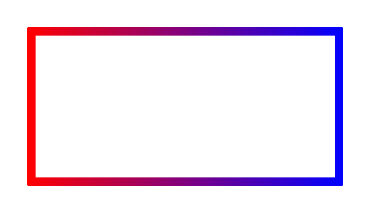
\begin{tikzpicture}
  \shade [left color=red,right color=blue] (-2,-1) rectangle (2,1);
  \begin{scope}[transparency group=knockout]
    \fill [white] (-1.9,-.9) rectangle (1.9,.9);
    \node [opacity=0,font=\fontencoding{T1}\fontfamily{ptm}\fontsize{45}{45}\bfseries]
          {Ti\emph{k}Z};
  \end{scope}
\end{tikzpicture}
\end{codeexample}
            %
            In the example, we first draw a large shading and then, inside the
            transparency group ``overwrite'' most of this shading by a big
            white rectangle. The interesting part is the text of the node,
            which has opacity |0|. Normally, this would mean that nothing is
            shown. However, in a knockout group, we ``paint'' the text with an
            ``opacity zero'' color. The effect is that part of the totally
            opaque white rectangle gets overwritten by a perfectly transparent
            area (namely exactly the area taken up by the pixels of the text).
            When this whole knockout group is then placed on top of the
            shading, the shading will ``shine through'' at the knocked-out
            pixels.

        \item \declare{|isolated|}|=false| A group can be isolated or not. By
            default, they are isolated, since this is typically what you want.
            For details on what isolated groups are, exactly, see Section~7.3.4
            of the \textsc{pdf} Specification, version~1.7.
    \end{itemize}

    Note that when a transparency group is created, \tikzname\ must correctly
    determine the size of the material inside the group. Usually, this is no
    problem, but when you use things like |overlay| or |transform canvas|,
    trouble may result. In this case, please consult
    Section~\ref{section-transparency} on how to sidestep this problem in such
    cases.
\end{key}


%%% Local Variables:
%%% mode: latex
%%% TeX-master: "pgfmanual"
%%% End:
